\chapter{Background}

\section{Cryptocurrencies}
Before going delving into the financial side of the project, it is important to understand the underlying assets and the technology that drive them.

\subsection{Blockchain}
The building blocks of cryptocurrencies comes from blockchain. Blockchain is a distributed ledger that stores data, in blocks, in a chain, comprising the data itself as well has a full transaction history~\cite{nofer2017blockchain}. Below shows a diagram of blocks in a blockchain.

\begin{figure}[!htb]
    \centering
    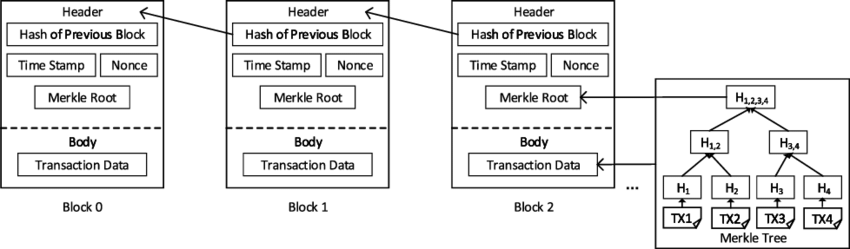
\includegraphics[width=0.8\textwidth]{background/Images/The-structure-of-a-Blockchain.png}
    \caption{Blockchain Diagram~\cite{inbookBlockchain}}
\end{figure}

\subsubsection{Header, Hash of Previous Block and Timestamp}
The timestamp and hashes of the block and its' predecessing block are all used to ensure the ordering of blocks within a chain. By hashing the data to a fixed size, and storing in its succeeding block makes the tampering of chains difficult as it would mean the chain deviates from its old state. In addition to this, by hashing and using Nonce, blockchain employs the Proof-of-Work algorithm to ensure correctness. The Proof-of-Work algorithm is used to confirm and add new transaction to the chain.

\subsubsection{Nonce}
A nonce, `Number Only used Once', is a number that is added to a hashed block to make the transaction more secure. It is randomly generated which miners use to validate a transaction. A miner first guesses a nonce, appends the guess to the hash of the current header. The miner then rehashes the value and compares this to the target hash. If the guess was correct, the miner is granted the block~\cite{noauthor_components_2021}.

\subsubsection{Merkle root}
A merkle root is also stored in each block to validate transactions in an efficient manner, in terms of storage and searching. A merkle tree is a a tree of hashes where each leaf node is it's data hash and it's parent node, the hash of their children's hashes. In storing the merkle root, we do not need to directly store each transaction in each block, and also allows a quick search for any malicious alterations in differing blocks~\cite{noauthor_merkle_nodate}.

\subsection{Decentralised Finance}
One of the first application of blockchain was by Satoshi Nakamoto to create the first `purely peer-to-peer version of electronic cash'~\cite{nakamoto2009bitcoin}. Nakamoto's solution details the process in which a decentralised, peer to peer approach to verify and track transactions without a centralized institution. Since then, many other technologies derived from using blockchain as its underlying technology. One of them was proposed by Vitalik Buterin, the co-founder of Ethereum, in a whitepaper that proposed the idea of using smart contracts to create financial products and services that could operate independently of traditional financial institutions, hence decentralised finance was birthed~\cite{buterin2014next}.

\subsubsection{Ethereum}
Ethereum's architecture is similar to bitcoin's but has a few differences, one of which is the blockchain contains a copy of the transaction list and the most recent state. The process of how transactions are validated is below:
\begin{enumerate}
    \itemsep0em
    \item Validate the parent block
    \item Validate that the current timestamp is greater that the previous timestamp
    \item Check that the Ethereum concepts are valid
    \item Perform Proof of Work on the block
    \item Check for errors and gas
    \item Validate the final state
\end{enumerate}

\noindent Proof-of-Work (PoW) is a consensus protocol that is used by Ethereum and Bitcoin for the entire network to agree on the state of the blockchain. This provides security from malicious users to attempt to altering, adding/removing transactions or maintaining a second chain, the blockchain as it requires for 51\% of the network to agree on the alteration. One of the main problems of PoW is that is uses a lot of energy, ethereum miners were collectively consuming about 70 TWh/yr~\cite{noauthor_proof--work_nodate}.
\\[5mm]
To measure how much computational effort is required to execute operations on the ethereum network, gas is used~\cite{noauthor_gas_nodate}. Every block has a base fee, derived from the demand for the block space, which is burnt. Therefore, users of the network are expected to set a tip (priority fee) to reimburse miners for adding their transaction in blocks, thus the higher the tip, the greater the incentive for miners to validate the transaction. Using gas means that the ethereum network is tolerant to spam and also has a maximum gas fee to make ethereum tolerant to malicious code that would be used to waste resources.
\\[5mm]
Another difference between Ethereum and other cryptocurrencies is that rather than managing a distributed ledger, it uses a distributed state machine. The Ethereum Virtual Machine (EVM) defines the rules of changing states from block to block. Each node on the Ethereum blockchain contains an immutable instance of the EVM~\cite{noauthor_ethereum_nodate}.

\begin{figure}[!htb]
    \centering
    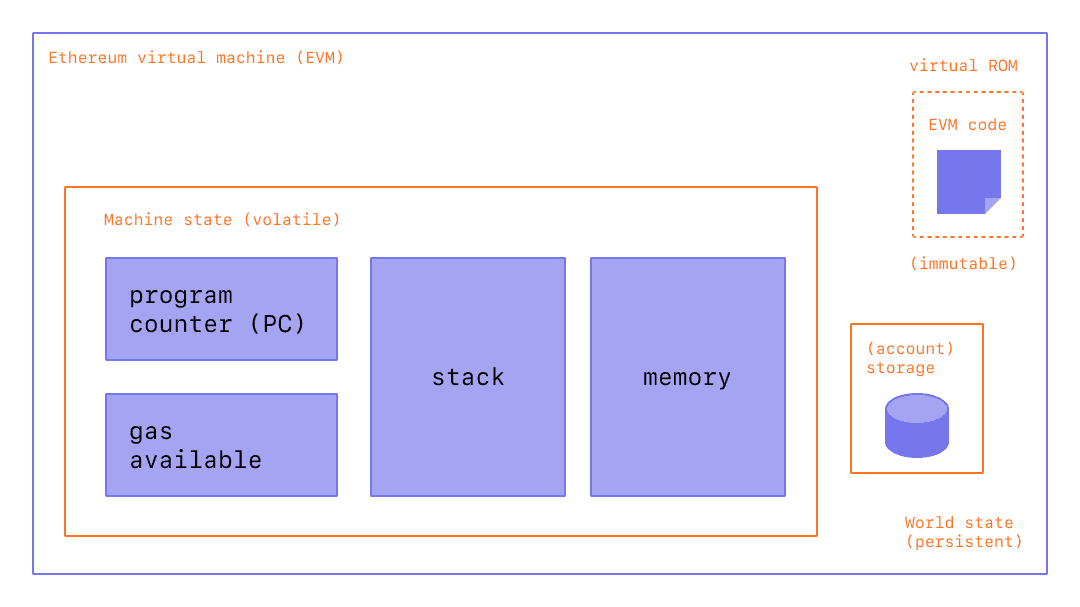
\includegraphics[width=0.8\textwidth]{background/Images/evm.png}
    \caption{EVM components~\cite{noauthor_ethereum_nodate}}
\end{figure}

\subsubsection{Smart Contracts}
Smart contracts are programs that are self-executing contracts between buyers and sellers that deploy on the ethereum network. It allows for the automation of a contract's execution, and can be used to facilitate, verify, and enforce the negotiation or performance of a contract~\cite{noauthor_introduction_nodate, noauthor_smart_nodate}.

\section{Arbitrage}
Arbitrage is the process in which a trader simultaneously buys and sells an asset in order to take advantage of a market inefficiency~\cite{businessinsightsblog_2021}. Arbitrage is also possible in other types of securities by finding price inefficiencies in the prices of options, forward contracts and other exotics.
\\[5mm]
Sources have shown that the word ``\textit{Arbitrage}'' has been used as early as the Renaissance era wehere surviving documents showed a large amount of bills being exchanged~\cite{poitras_2021}. There has also been some evidence to suggest that arbitrage was used as early as the Greek and Roman eras. Objects such as Sumerian cuneiform tablets show trade of ancient bills however we cannot come to strong conclusions of this. Early forms of arbitrage would likely to have been purchasing a commodity then transporting them to a foreign land and selling them at a higher price. This is type of arbitrage is called commodity arbitrage and is still is applicable today. With the example above, transporting the goods takes a significant amount of to the merchant, trader, which could cause variations in the price, however in the modern day this has been reduced and with electronic exchanges this time to buy and sell is very small. This means inefficiencies in the market, where a trader can profit purely by buying and selling, should not exist. This is called the ``Law of One Price''. The ``Law of One Price'' states that every identical commidty or asset should have the same price regardless of exchange or location, given there are no transaction costs, no transportation costs, no legal restrictions, the exchange rates are the same and no market manipulation occurs~\cite{noauthor_law_nodate}. This is because if this were not the case, an arbitrage opportunity would arise and someone would take advantage of the scenario causing the prices on both markets to converge due to the market forces. In the real world arbitrage opportunities are tremendously common, thus allowing a risk-free investment~\cite{10.2307/1828075, RICHARDSON1978341}.
\\[5mm]
There are countless types of arbitrage such as spatial arbitrage, which profits off of different prices on exchanges in different locations, temporal arbitrage, which takes advantage of price differences at different times, risk arbitrage, which proifts from perceived discrepancies in their risk-return profiles and finally market arbitrage which takes advantages of different prices on different exchanges/markets. Statistical methods include pairs trading, which involves buying and selling assets that are believed to be mispriced relative to one another, momentum trading, which identifies if assets have a strong momentum (either up or down) and profiting off of that, and finally algorithmic trading which uses algorithms to analyze data and trades based on statistical analysis. This project shows how these opportunities can be exploited both in a pure manner as well as using statistical methods.

\section{State of Art}
To better understand the project and to be able to research into something new and novel it is important to understand the current state of art, i.e. previous research on the topic. Research into cryptocurrency arbitrage is still in its infancy and previous research has mainly focussed on the economics of cryptocurrencies, i.e. miner/trader behaviour and influence of cryptocurrency trading~\cite{eyal2015miner, avarikioti2020ride, huberman2021monopoly, athey2016bitcoin, easley2019mining, harvey2016cryptofinance, pagnotta2018equilibrium}. Furthermore, there has been very limited research in comparing statistical strategies and pure methods of arbitrage of cryptocurrencies. Despite this, there has been plentiful research on arbitrage as a whole as it is immensly profitable, as a result of this people/institutions tend to keep their newly found research secret. Of the published research, I have looked into the arbitrage techniques that are used. As arbitrage can is highly profitable, it can be found in countless types or assets, such as options, stocks, bonds and many other types of products. Research into all types of products exist going into the theory and practical aspects of each \cite{mo_theoretical_nodate, 8957853}. The most similar type of asset class to cryptocurrencies is fiat currencies, such as the US Dollar and the Great British Pound Sterling. The research in arbitrage in foreign exchanges show that using a triangular/cyclic arbitrage is highly profitable and effective~\cite{akram2008arbitrage, aiba2002triangular, ito2012free}. 

\subsection{Pure Arbitrage Techniques}
As I am using pure arbitrage as a baseline, thus choosing the most optimal stategy is most ideal to better understand the impacts of the optimizations and the statistical stategies themselves. There has been some research on pure arbitrage strategies by finding cyclic opportunities on both centralized and decentralised exchanges, which I go further into in this section.
\\[5mm]
As previously mentioned, research into this topic is still in its infancy thus which means a very thin slice of exploration on the subject matter. Majority of the research has been into the arbitrage on centralized exchanges,~\cite{MakarovIgor2020Taai, crepelliere_arbitrage_2022, PAUNACristian2018ATSf}. These all find massive inefficiencies within these exchanges by finding arbitrage opportunities. One of the more in depth pieces of research, Igor Makarov's and Antoinette Schoar's Trading and arbitrage in cryptocurrency markets~\cite{MakarovIgor2020Taai} finds a large violation in the Law of One Price by finding price discrepencies between the same cryptocurrencies depending on different geolocations. The paper uses 34 exchanges in 19 differing countries, each exchange is grouped accordingly to its location and base currencies, leaving China, Japan, Korea, US, Europe and another group for that uses the Tether, USDT. Within each group the arbitrage index is calculated to compare the maximum difference in prices between exchanges within the same exchange group. This is done by calculating the volume-weighted average price at each exchange, then dividing the maximum price by the minimum price thus if the arbitrage index is 1, then there does not exist an arbitrage opportunity. It is shown that the arbitrage index is over 1 most of the time in all regions thus show a large amount of arbitrage opportunities across different exchanges, with opportunities lasting for as long as several weeks. It is also shown that the arbitrage spreads are consistent and correlated between regions and countries. Although the paper goes into some detail about how one can go about implementing such strategies and it's complications, it didn't implement them thus provides a simply theoretical hypothesis that may or may not work in practice.
\\[5mm]
Cristian Pauna implements an arbitrage strategy in~\cite{PAUNACristian2018ATSf}. The paper details the technical details of arbitrage trading from the data and the system architecture used. Pauna finds complications such as requesting data from multiple exchanges, converting the data such that it is homogeneous and also managing server load. Pauna presents the architecture such that the servers request data from the necessary exchanges, stores them in a relational database which then triggers a server that is used to generate trading signals.

\begin{figure}[!htb]
    \centering
    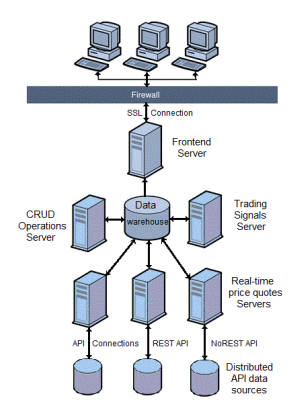
\includegraphics[width=0.28\textwidth]{background/Images/Arbitrage-Architecture.png}
    \caption{Arbitrage system architecture~\cite{PAUNACristian2018ATSf}}
\end{figure}

Now looking at DEXs, research done by Stephen Bryne in his paper,~\cite{byrneexploration} introduces other methods that are commonly used however, not been academically been explored. Methods using properties of ethereum such as using smart contracts for flash loans and buying and selling the same asset in large volumes within the same block in the chain, leading to large profits. The paper details into the technical implementations and issues such as security and reliablity, however it fails to provide analysis and quantitative results on the different methods used to exploit arbitrage opportunities and their differences.
\\[5mm]
As previously mentioned triangular and cyclic arbitrage is one of the most used and purest forms of arbitrage to implement and analyse,~\cite{boonpeam2021arbitrage} explores triangular arbitrage on decentralised exchanges. Algorithm \ref{alg:arb_sys_on_dex} is the algorithm used to find the most profitable arbitrage route on a particular platform, once this is calculated, it is compared with other routes on other platforms. Initially, the system converts the base token into another token and converts it back into the base token, using only one token is used as a middle route, then using the algorithm below, increases the number of middle tokens.

\begin{algorithm}
    \caption{Maximum Profit Route Searching (R)}\label{alg:arb_sys_on_dex}
    \textbf{Input}: $T$ (token list), $P$ (price graph), $n$ (current route)
    \begin{algorithmic}
    \For{$i = 1, ..., T$}
        \State $r = get\_profit(n+i)$
        \For{$j = 1,...,P[i]$}
            \State $p = max(r, R(T, P, n_j))$
        \EndFor
    \EndFor
    \State \textbf{return} $p$
    \end{algorithmic}
\end{algorithm}

\noindent On evaluating the performance of the strategy on differing platforms depended on three main features of each exchange:
\begin{enumerate}
    \item Portion size - Depending on how much the ``trader'' invested revenues differed and infact the larger protion size the revenue decreases as the token pair prices are adjusted based on supply/demand.
    \item Transaction fees - Each exchange has their own transaction fee.
    \item Other considerations such as price slippage - Exchanges have different liquidity levels which depends on the usage and liquidity providers that the exchange employs.
\end{enumerate}

It is found that using this strategy out of the exchanges; Uniswap, 1inch, Kyberswap and Bancor. 1inch was the only exchange that generated a profit whereas the others lose money. The results are shown below on the revenues recieved on each platform experimented on.

\begin{figure}[!htb]
    \centering
    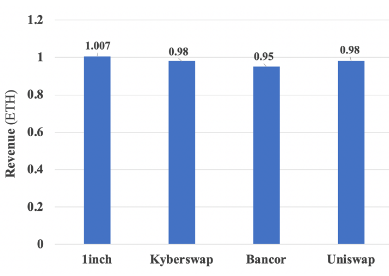
\includegraphics[width=0.5\textwidth]{background/Images/DEXArb_results.png}
    \caption{Trading revenues same token routes within different exchange~\cite{boonpeam2021arbitrage}}
\end{figure}

Another paper that implemented and evaluated a cyclic arbitrage opportunity is~\cite{wang_cyclic_2022}. The research consists of proposing a theoretical arbitrage model and further evaluation on real transactional data. The arbitrage model used is simple to understand, as it searches for a cyclic transaction between $n$ tokens, $A_1, A_2, ..., A_n$ is a sequence of $n$ trades:
\begin{center}
    \begin{minipage}[c]{0.4\linewidth}
    \begin{itemize}
        \item[\textit{Trade 1:}] Exchange $\delta_1$ of $A_1$ to $\delta_2$ of $A_2$
        \item[\textit{Trade 2:}] Exchange $\delta_2$ of $A_2$ to $\delta_3$ of $A_3$
        \item[] $\dotsc$
        \item[\textit{Trade n:}] Exchange $\delta_n$ of $A_n$ to $\delta_1'$ of $A_1$
    \end{itemize}
    \end{minipage}
\end{center}

It is important to note that $\delta_i = \delta_{i+1}$, i.e. the output of a trade is equivelent to the input of the next. The revenues within a cycle are defined as $\delta_{i+1} - \delta_i$, and the overall profit is $\delta_{1}' - \delta_1$. This is not as simple as the revenues obviously depend on how liquid the exchange is, thus the liquidity pools of each possible trading pair is hugely important. Therefore, the paper proposes a theorem, below:

\begin{theorem}
    For a given cycle $A_1 \rightarrow A_2 \rightarrow \cdots \rightarrow A_n \rightarrow A_1$ with $n$ tockens, there exists an arbitrage opportunity for the cyclic transaction if the product of exchange rates $\frac{a_{2,1}a_{3,2}\cdots a_{1,n}}{a_{1,2}a_{2,3}\cdots a_{n, 1}} > \frac{1}{r_1^n r_2^n}$ where $a_{i,j}$ denotes the liquidity of token $A_i$ in the liquidity pool with token $A_j$.~\cite{wang_cyclic_2022}
\end{theorem}

In addition to the theorem, to obtain an optimal strategy we need to compute the optimal trading volume of a cycle, $A_1 \rightarrow A_2 \rightarrow \cdots \rightarrow A_n \rightarrow A_1$. The paper proposes the optimal trading volume to be $\delta^{op}_a = \frac{\sqrt{r_1 r_2 a' a} - a}{r_1}$ where $a = \frac{a_{1,n}'a_{n,1}}{a_{n,1}+r_1 r_2 a_{n,1}'}$ and $a' = \frac{r_1 r_2 a_{1,n}'a_{n,1}}{a_{n,1}+r_1 r_2 a_{n,1}'}$. Thus in order to calculate such arbitrage opportunities knowing the liquidity of tokens in other tokens' liquidity pools, algorithm \ref{alg:liquidity_alg} infers the direction and volumes to trade to get the optimal revenue.

\begin{algorithm}
    \caption{Computing the equivelent liquidity of the cycle}\label{alg:liquidity_alg}
    \begin{algorithmic}
        \State $a_{1, n}' \leftarrow a_{1,2}$
        \State $a_{n, 1}' \leftarrow a_{2,1}$
        \For{$i$ from $2$ to $n-1$}
            \State $a_{1, n}' \leftarrow \frac{a_{1,n}'a_{i,i+1}}{a_{i,i+1}+r_1 r_2 a_{n,1}'}$
            \State $a_{n, 1}' \leftarrow \frac{r_1 r_2 a_{1,n}'a_{i+1, i}}{a_{i,i+1}+r_1 r_2 a_{n,1}'}$
        \EndFor
    \end{algorithmic}
\end{algorithm}

After analysis, it is found that between 4th May 2020 to 15th April 2021, there were countless exploitable arbitrage opportunities and in fact grew to 1,750 in the 11 months that it was tested on. Only cycles with length 3 were experimented with and only cycles including ETH as 80\% of the liquidity pools on Uniswap include ETH and another cryptocurrency~\cite{heimbach2021behavior}. Furthermore, it is found that 287,241 of the 292,606 arbitrages executed started with ETH, 85\% of the arbitrages used a cycle of length 3. The total revenue of the cyclic arbitrage was 34,429 ETH. However, gas fees accounts for 24.6\% of the total revenue leaving an approximate 25,971 ETH profit.
\\[5mm]
% \vspace{5mm}
The paper then delves into the implementation of the smart contract, the paper explored how both \textit{sequential} and \textit{atomic} implementations would affect the revenue and execution of the contracts. It was found that 52.3\% of the arbitrages that were executed sequentially generated a loss, likely due to the fact when one submits $n$ orders, the $n$ blockchain transactions are executed sequentially, meaning some external transactions can be inserted between these transactions. Thus using atomic transactions avoids this issue of external transactions do not effect the market price that may effect the outcome of the arbitrage.
\\[5mm]
Furthermore, the authors of the paper also investigated the performance differences of using private smart contracts and public contracts. Deploying a smart contract that calls Uniswap functions, i.e. a private smart contract, is intuitively better and achieves a higher success rate of a lower bound of 52\% and a higher bound of 90\% in comparison to calling a public Uniswap smart contract which has success rate of 27.3\%. Overall the paper provides an insightful look into cyclic arbitrage in DEXs and highlights important decisions made such as liquidity calculations and smart contracts, while comparing the performance of differing options available.

\subsection{Statistical Arbitrage Techniques}

As mentioned previously mentioned and the subject of the project is to optimize statistical arbitrage methods to be able to compete with a more purer form of arbitrage, i.e. cyclic arbitrage. As previously mentioned there are many methods of stat arb, pairs trading, momentum trading and algorithmic trading. Within these methods there are countless strategies to adopt and profit off of, thus to limit the scope, this project I will be investigating strategies within pair trading. Research within Pair trading has been vast with many streams of approaches emerging; distance approach, cointegration approach, time-series approach, stochastic approach and some others, including using machine learning~\cite{https://doi.org/10.1111/joes.12153}. 
\\[5mm]
The distance approach is easy to understand; using the euclidian squared difference of combinations historical normalized prices of assets from a selected time period and selecting the top 20 pairs of assets with the least historical distance. Once pairs are selected, monitor the prices and if the prices diverge by over 2 standard deviations, buy the undervalued asset and sell the overvalues asset and when the prices converge, close the position~\cite{RadLowFaff}. This is called Mean reversion and is fundemental technique used in pairs trading.
\\[5mm]
The cointegration approach follows three key steps. The first being selection of pairs based on similarity measures, the next being assessing the tradability and finally thresholds are set for trading. The spread is defined as $$\varepsilon_{i j,t} = P_{i,t} + \gamma P_{j,t}$$ where $P_{i,t}$ and $P_{j,t}$ denote the $I(1)$ non-stationary price processes of the assets $i$ and $j$, $\gamma$ is the cointegration coefficient, also refered to in literature as the hedge ratio. $\varepsilon_{i j,t}$ is the linear combination of the non-stationary prices and is $I(0)$ stationary and hence mean-reverting, note that stationary processes are those of which have a constant mean. Rad's implementation of this approach on stocks result in a 0.83\% return before considering transaction costs~\cite{RadLowFaff}. Another paper, \cite{lossProtection}, looked into setting the thresholds and setting a minimum profit, $MP_{ij,t_c}$: $$MP_{ij,t_c} = \frac{n(\varepsilon_{i j,t_0} - \varepsilon_{i j,t_c})}{ \mid \gamma \mid}$$ Where $t_0$ and $t_c$ are the opening and closing times, $n$ is the volume longed of asset $j$.
\\[5mm]
There has been further research into optimizing mean reversion, one of which was to use the successive convex approximation method on the mean reverting portfolio design ~\cite{ZipingZhao2019OMPW}. The paper initially proposes the mean reversion portfolio:
\begin{itemize}
    \itemsep0em
    \item For each asset, the price at time $t$ is denoted as $p_t$ and its correspondeing log-price $y_t \triangleq log(p_t)$, its vector form of $M$ assets $\mathbf{y}_t \triangleq \big[ y_{1,t}, \dots ,w_{M,t} \big]^T$.
    \item The log-price spread is given by $y_t \triangleq \mathbf{\beta}^T\mathbf{y}_t$, where $\mathbf{\beta} \triangleq \big[ \beta_1, \dots ,\beta_M \big]^T$ denotes the hedge ratios.
    \item The cointegration space with $N$ relations is defined by $\mathbf{B} \triangleq \big[ \beta_1, \dots ,\beta_N \big]$, thus the $N$ spreads are $s_t \triangleq \mathbf{B}^T\mathbf{y}_t$.
    \item For these $N$ spreads, the portfolio weight matrix is denoted as $\mathbf{w} \triangleq \big[ w_1, \dots ,w_N \big]^T$.
    \item The auto-covariance matrix for the spreads $s_t$ is defined as \\ ${M_i \triangleq Cov(s_t, s_{t+i}) = \mathop{\mathbb{E}} \big[ \big( s_t - \mathop{\mathbb{E}} \big[ s_t \big]\big) \big( s_{t+i} - \mathop{\mathbb{E}} \big[ s_{t+i} \big]\big)^T \big]}$
\end{itemize}

Now that we have defined everything required, we can now formulize the problem. The general problem of mean reversion portfolio design problem is formalized by:
\begin{equation*}
    \begin{aligned}
        & \underset{\mathbf{w}}{\text{minimize}}
        & & F(\mathbf{w}) \triangleq U(\mathbf{w}) + \mu V(\mathbf{w}) + \gamma S(\mathbf{w})\\
        & \text{subject to}
        & & \mathbf{w} \in \biggl\{ \mathbf{w} \mid \big\| \mathbf{B} \mathbf{w}\big\|_0 \leq L \biggr\}, \qquad \text{where $L$ is the total leveraged investment}
    \end{aligned}
\end{equation*}

\noindent Where the Mean Reversion term: $$U(\mathbf{w}) \triangleq \xi \frac{\mathbf{w}^T \mathbf{H}\mathbf{w}}{\mathbf{w}^T \mathbf{M}_0\mathbf{w}} + \zeta \biggl( \frac{\mathbf{w}^T \mathbf{M}_1\mathbf{w}}{\mathbf{w}^T \mathbf{M}_0\mathbf{w}} \biggr) ^2 + \eta \sum_{i=2}^{p} \biggl( \frac{\mathbf{w}^T \mathbf{M}_i\mathbf{w}}{\mathbf{w}^T \mathbf{M}_0\mathbf{w}}\biggr)^2$$ And the variance term: $$V(\mathbf{w}) \triangleq \begin{cases}
    1/\mathbf{w}^T \mathbf{M}_0\mathbf{w} & \text{VarInv(\textbf{w})}\\
    1/\sqrt{\mathbf{w}^T \mathbf{M}_0\mathbf{w}} & \text{StdInv(\textbf{w})}\\
    -\mathbf{w}^T \mathbf{M}_0\mathbf{w} & \text{VarNeg(\textbf{w})}\\
    -\sqrt{\mathbf{w}^T \mathbf{M}_0\mathbf{w}} & \text{StdNeg(\textbf{w})}
 \end{cases}$$ 
 The variance term can be represented in any of the four forms.
 \\[5mm] 
 And the asset selection term: $$S(\mathbf{w}) \triangleq \big\| \mathbf{B} \mathbf{w}\big\|_0 = \sum_{m=1}^{M} sgn(\mid \bigl[ \mathbf{B} \mathbf{w} \bigr]_m \mid)$$ This asset selection critorian is not necessary however as trading incur a cost, selecting all of the asset is costly, thus selecting a subset of assets to trade is more profitable. To formulize this goal, we would like to minimize the cointegration space thus we use the $\ell_0$ norm.
 
 Where \begin{itemize}
    \item $\mu$ defines the trade-off between the mean reversion measure and the variance preference.
    \item $\gamma$ defines the regularization parameter of how sparse we would like the cointegration space to be.
 \end{itemize}



\textbf{Ones that use Cointegration/Correlation:}
\begin{itemize}
    \item OPTIMAL PORTFOLIO DESIGN FOR STATISTICAL ARBITRAGE IN FINANCE \cite{8450775} %file:///home/devam/Documents/Imperial/Year_4/Individual%20Project/Interim%20Report/background/Articles/Optimal_Portfolio_Design_for_Statistical_Arbitrage_in_Finance.pdf
    % \item Optimal Mean-Reverting Portfolio With Leverage Constraint for Statistical Arbitrage in Finance \cite{ZipingZhao2019OMPW} %file:///home/devam/Documents/Imperial/Year_4/Individual%20Project/Interim%20Report/background/Articles/Optimal_Mean-Reverting_Portfolio_With_Leverage_Constraint_for_Statistical_Arbitrage_in_Finance.pdf
    \item Exploring sources of statistical arbitrage opportunities among Bitcoin exchanges \cite{KRISTOUFEK2023103332} %file:///home/devam/Documents/Imperial/Year_4/Individual%20Project/Interim%20Report/background/Articles/Exploring_sources_of_statistical_arbitrage_opportunities_among_bitcoin_exchanges.pdf
    \item Common dynamic factors for cryptocurrencies and multiple pair-trading statistical arbitrages \cite{Figa-TalamancaGianna2021Cdff} %file:///home/devam/Documents/Imperial/Year_4/Individual%20Project/Interim%20Report/background/Articles/Common%20dynamic%20factors%20for%20cryptocurrencies%20and%20multiple%20pair-trading%20statistical%20arbitrages.pdf
\end{itemize}


\textbf{Ones that use Kalman Filter:}
\begin{itemize}
    \item A Combination Forecasting Model Using Machine Learning and Kalman Filter for Statistical Arbitrage \cite{6974093} %file:///home/devam/Documents/Imperial/Year_4/Individual%20Project/Interim%20Report/background/Articles/A_combination_forecasting_model_using_machine_learning_and_Kalman_filter_for_statistical_arbitrage.pdf
    \item Pairs Trading with a Kalman Filter \cite{dempsey_market_2017} %file:///home/devam/Documents/Imperial/Year_4/Individual%20Project/Interim%20Report/background/Articles/Pairs%20Trading%20with%20a%20Kalman%20Filter.pdf
\end{itemize}





% \newpage
% \textbf{Broader Picture}
% \begin{itemize}
%     \item STATISTICAL ARBITRAGE PAIRS TRADING STRATEGIES: REVIEW AND OUTLOOK \cite{https://doi.org/10.1111/joes.12153} %file:///home/devam/Documents/Imperial/Year_4/Individual%20Project/Interim%20Report/background/Articles/Journal%20of%20Economic%20Surveys%20-%202016%20-%20Krauss%20-%20STATISTICAL%20ARBITRAGE%20PAIRS%20TRADING%20STRATEGIES%20REVIEW%20AND%20OUTLOOK.pdf
%     \item Statistical Arbitrage: Algorithmic Trading Insights and Techniques \cite{alma991000607977501591} %file:///home/devam/Documents/Imperial/Year_4/Individual%20Project/Interim%20Report/background/Articles/Statistical%20arbitrage%20:%20algorithmic%20trading%20insights%20and%20techniques.pdf
% \end{itemize}


%%%%%%%%%%%%%%%%%%%%%%%%%%%%%%%%%%%%%%%%%%%%%%%%%%%%%%%%%%%%%%%%%%%%%%%%%%%%%%%%%%%%%%%%%%%%%%%%%%%%%%%%%%%%%%%%%%%%%%%%%%%%%%%%%%%%%%%%%%%%%%%%%%%%%%%%%%%%%%%%%%%%%%%%%%%%%%%%%%%%%%%%%%%%%%%%%%%%%%%%%%%%%%%%%%%%%%%%%%%%%%%%%%%%%%%%%%%%%%%%%%%%%%%%%%%



\textbf{Ones that use Stochastics:}
\begin{itemize}
    \item Statistical Arbitrage with Pairs Trading \cite{GoncuAhmet2016SAwP} %file:///home/devam/Documents/Imperial/Year_4/Individual%20Project/Interim%20Report/background/Articles/Statistical%20Arbitrage%20with%20Pairs%20Trading.pdf
\end{itemize}


\textbf{Ones that use ML:}
\begin{itemize}
    \item Statistical Arbitrage in Cryptocurrency Markets \cite{jrfm12010031} %file:///home/devam/Documents/Imperial/Year_4/Individual%20Project/Interim%20Report/background/Articles/Statistical%20Arbitrage%20in%20Cryptocurrency%20Markets%20.pdf
    \item Deep neural networks, gradient-boosted trees, random forests: Statistical arbitrage on the S\&P 500 \cite{KRAUSS2017689} %file:///home/devam/Documents/Imperial/Year_4/Individual%20Project/Interim%20Report/background/Articles/Deep_neural_networks,gradient-boosted_trees,random_forests:_Statistical_arbitrage_on_the_S&P_500.pdf
    \item A Machine Learning based Pairs Trading Investment Strategy \cite{alma991000475380901591} %file:///home/devam/Documents/Imperial/Year_4/Individual%20Project/Interim%20Report/background/Articles/A%20Machine%20Learning%20based%20Pairs%20Trading%20Investment%20Strategy%20.pdf
\end{itemize}




% WowSwap, dydx, gmx, ... https://defiprime.com/margin-trading
% https://corporatefinanceinstitute.com/resources/cryptocurrency/cryptocurrency-exchanges/
% https://wowswap-io.medium.com/the-big-short-introducing-decentralized-leveraged-short-swaps-a81eb9d1c36f 
% https://defiprime.com/margin-trading
% https://github.com/evbots/dex-protocols
% 
% https://medium.com/defi-saver/how-to-long-or-short-any-asset-using-defi-lending-protocols-812300c9a640
% https://defiprime.com/exchanges

% https://www.youtube.com/watch?v=zABaCh3yAho - video on markovian auto regressive methods
% https://medium.com/@rachita.pateria/an-introduction-to-markov-switching-model-for-time-series-b279e9e26125

% \begin{enumerate}
%     \item \cite{HuangJianfeng2022Taaf} - %https://library-search.imperial.ac.uk/permalink/44IMP_INST/fv0fdm/cdi_informaworld_taylorfrancis_310_1080_13504851_2021_1930998
%     \item \cite{alma991000411969901591} - %https://library-search.imperial.ac.uk/permalink/44IMP_INST/mek6kh/alma991000411969901591
%     \item \cite{} - %https://library-search.imperial.ac.uk/permalink/44IMP_INST/mek6kh/alma991000343762601591
%     \item \cite{} - %https://library-search.imperial.ac.uk/permalink/44IMP_INST/mek6kh/alma996037714401591
%     \item \cite{} - %https://library-search.imperial.ac.uk/permalink/44IMP_INST/mek6kh/alma991000617323401591
% \end{enumerate}












